\chapter{Computational Study}\label{comp_study}
In this chapter, the model presented in \Cref{model} has been implemented in Python with the use of
the Gurobi Python solver.  The model has been run with instances described in Chapter \ref{case_study} on a computer with the specifications presented in \Cref{comp_study_specs}.
\\
\begin{table}[H]
    \centering
    \caption{Specifications of computer, solver, and programming language.}
    \begin{tabular}{l| l}
        Processor & 4x 2.2GHz AMD Opteron 6274 – 16 core\\
        RAM & 128GB \\
        Operating System & CentOS 7.8.2003 \\
        Guribi version & 3.7.9\\
        Python version & 9.1.0\\
    \end{tabular}
    \label{comp_study_specs}
\end{table}

\Cref{prelim_study} analyzes the different symmetry-breaking constraints and valid inequalities presented in \Cref{model}. Furthermore, the size of solvable instances and parameters affecting computational time is evaluated in \Cref{tech_analysis}, whereas \Cref{econ_analysis} estimates how parameters
change the quality of solutions from an economic point of view. Finally, \Cref{comp_models} compares the alternative model proposed in \Cref{alt_model} with the model presented in \Cref{model}.


\section{Preliminary Study}\label{prelim_study}

The team orienteering problem is NP-complete \citep{golden_orienteering_1987} and, therefore it has an enormous solution space even for small instances. In this subsection, an evaluation of the different constraints introduced in \Cref{model} is done. These constraints tighten the solution space and improve computational time. Three instances are defined to compare the different constraints. The characteristics of these instances are presented in \Cref{computational_preliminary}. Test data for these instances are generated as described in \Cref{gen_test_inst}, with parameters aimed at solving the instances in a reasonable amount of time.
\\
\begin{table}[H]
    \centering
    \caption{Characteristics of instances tested in preliminary study}
    \begin{tabular}{l c c c c}
        \thickhline
        \textbf{Parameters} & \textbf{Instance 1} & \textbf{Instance 2}  & \textbf{Instance 3} \\
        \thickhline
        \textbf{Scooters per zone} & 4 & 4 & 5 \\
        \textbf{Service vehicles} & 2 & 3 & 2 \\
        \textbf{Shift duration} & 17 & 17 & 17 \\
        \thickhline
        \end{tabular}
    \label{computational_preliminary}
\end{table}


\subsection{Symmetry-Breaking Constraints}\label{prelim_sym_break}

The base model, given by constraints \eqref{eq:const_deopt}-\eqref{eq:const_vcap_depot_in}, is the foundation of all the model variants in this study. As the problem is defined with a homogeneous fleet, practical equal solutions can be excluded by adding symmetry-breaking constraints \eqref{eq:const_number_of_arcs}-\eqref{eq:const_total_time_used}. The three symmetry-breaking constraints introduced in \Cref{model} limit the number of arcs traveled \eqref{eq:const_number_of_arcs}, the number of visits \eqref{eq:const_number_of_visits}, or total time used \eqref{eq:const_total_time_used} by vehicle $v$ to break the symmetry properties of the problem. 
\\
\begin{table}[H]
    \centering
    \caption{Variants of symmetry-breaking constraints in preliminary study}
    \begin{tabular}{c c l}
        \thickhline
        \textbf{Name} & \textbf{Constraints} & \textbf{Explanation}\\
        \thickhline
        \textbf{A} & (\ref{eq:const_deopt}) - (\ref{eq:const_vcap_depot_in}) & No symmetry-breaking constraints\\
        \textbf{B} & \textbf{A} + (\ref{eq:const_number_of_arcs}) & Number of arcs used by vehicle $v$ \\
        \textbf{C} & \textbf{A} + (\ref{eq:const_number_of_visits}) & Number of visits by vehicle $v$\\
        \textbf{D} & \textbf{A} + (\ref{eq:const_total_time_used}) & Total time used by vehicle $v$\\
        \thickhline
        \end{tabular}
    \label{variants_symmetry_preliminary}
\end{table}

Different variants of the model are presented in \Cref{variants_symmetry_preliminary}, and the performance of these models are presented in \Cref{results_symmetry_preliminary}. The symmetry-breaking constraint comes in handy when the number of vehicles increases from 2 to 3 in Instance 2. However, when the number of locations per zone changes from 4 to 5 in Instance 3, there is no significant improvement by adding the symmetry-breaking constraints. Model C is the overall best performer of the models with symmetry-breaking constraints and is therefore included in testing the valid inequalities. 
\\
\begin{table}[H]
    \centering
    \caption{Results from preliminary study with symmetry-breaking constraints}
    \begin{tabular}{c c c c c c c}
        \thickhline
         & \multicolumn{2}{c}{\textbf{Instance 1}} & \multicolumn{2}{c}{\textbf{Instance 2}} & \multicolumn{2}{c}{\textbf{Instance 3}}  \\
        \thickhline
        \textbf{Model variant} & Solution Time & Gap & Solution Time & Gap & Solution Time & Gap \\
        \hline
        \textbf{A} & 27 s & 0 \% & 523 s & 0 \% & 594 s & 0 \% \\
        \textbf{B} & 30 s & 0 \% & 349 s & 0 \% & 633 s & 0 \% \\
        \textbf{C} & \textbf{25 s} & \textbf{0 \%} & \textbf{268 s} & \textbf{0 \%} & \textbf{508 s} & \textbf{0 \%} \\
        \textbf{D} & 44 s & 0 \% & 218 s & 0 \% & 564 s & 0\% \\
        \thickhline
        \end{tabular}
    \label{results_symmetry_preliminary}
\end{table}

\subsection{Valid Inequalities}\label{prelim_val_ineq}

The three valid inequalities presented in \Cref{model} have been introduced to improve the computational time. Constraints (\ref{eq:const_back_and_forth}) and (\ref{eq:const_arcs_less_then_locations}) are implemented as stated in \Cref{model}, while the size of subsets in constraint (\ref{eq:const_subtour_in_set}) have been narrowed to 3, due to the huge amount of constraints. \Cref{variants_valid_inequalities_preliminary} summarizes the different variants of the model with valid inequalities and symmetry-breaking constraints \eqref{eq:const_number_of_arcs}. 
\\
\begin{table}[H]
    \centering
    \caption{Variants of valid inequalities in preliminary study}
    \begin{tabular}{c c l}
        \thickhline
        \textbf{Name} & \textbf{Constraints} & \textbf{Explanation}\\
        \thickhline
        \textbf{A} & (\ref{eq:const_deopt}) - (\ref{eq:const_vcap_depot_in}) & No symmetry-breaking constraints or valid inequ.\\
        \textbf{E} & \textbf{A} + (\ref{eq:const_back_and_forth}) & No back and forth between two locations \\
        \textbf{F} & \textbf{A} + (\ref{eq:const_subtour_in_set}) & Subtour elimination in subset\\
        \textbf{G} & \textbf{A} + (\ref{eq:const_arcs_less_then_locations}) & Number of arcs less than or equal number of locations\\
        \textbf{H} & \textbf{A} + (\ref{eq:const_subtour_in_set}) - (\ref{eq:const_arcs_less_then_locations}) & Number of arcs + subtour elimination in subset\\
        \textbf{I} & \textbf{A} + (\ref{eq:const_number_of_visits}), (\ref{eq:const_subtour_in_set}) & Subtour elimination + symmetry-breaking on visits\\
        \textbf{J} & \textbf{A} + (\ref{eq:const_number_of_visits}), (\ref{eq:const_arcs_less_then_locations}) & Number of arcs + symmetry-breaking on visits\\
        \textbf{K} & \textbf{A} + (\ref{eq:const_number_of_visits}), (\ref{eq:const_subtour_in_set}) -  (\ref{eq:const_arcs_less_then_locations}) & Number of arcs, subtour elim. + sym.-break. visits\\
        \thickhline
        \end{tabular}
    \label{variants_valid_inequalities_preliminary}
\end{table}

Results of the different model variants tested on the three predefined instances are presented in \Cref{results_valid_inequalities_preliminary}. All model variants performed equal or better than the base model when a vehicle was added. The main difference materialized when the number of e-scooters per zone was increased. Combining the valid inequalities with symmetry-breaking constraints yields the worst results. This might be due to the larger simplex tableau to be solved at every node in the branch and bound tree. Variant F and G surpassed the other variants in this study, but G gets highlighted as the winner considering the variant only adds one constraint to the model. As for further research in this chapter, the testing is performed on model G due to the fact that valid inequality has a better opportunity for scaling than symmetry-breaking constraints. 
\\
\begin{table}[H]
    \centering
    \caption{Results from preliminary study with valid inequalities}
    \begin{tabular}{c c c c c c c}
        \thickhline
         & \multicolumn{2}{c}{\textbf{Instance 1}} & \multicolumn{2}{c}{\textbf{Instance 2}} & \multicolumn{2}{c}{\textbf{Instance 3}}  \\
        \thickhline
        \textbf{Model variant} & Solution Time & Gap & Solution Time & Gap & Solution Time & Gap \\
        \hline
        \textbf{A} & 27 s & 0 \% & 523 s & 0 \% & 594 s & 0 \% \\
        \textbf{E} & 28 s & 0 \% & 406 s & 0 \% & 741 s & 0 \% \\
        \textbf{F} & 29 s & 0 \% & 285 s & 0 \% & 521 s & 0 \% \\
        \textbf{G} & \textbf{32 s} & \textbf{0 \%} & \textbf{217 s} & \textbf{0\%} & \textbf{559 s} & \textbf{0 \%} \\
        \textbf{H} & 32 s & 0 \% & 350 s & 0 \% & 965 s & 0 \% \\
        \textbf{I} & 46 s & 0 \% & 331 s & 0 \% & 646 s & 0 \% \\
        \textbf{J} & 31 s & 0 \% & 443 s & 0 \% & 761 s & 0 \% \\
        \textbf{K} & 70 s & 0 \% & 558 s & 0 \% & 761 s & 0 \% \\
        
        \thickhline
        \end{tabular}
    \label{results_valid_inequalities_preliminary}
\end{table}


\subsection{Relaxation of Integer Variables}\label{prelim_int_var_relax}

To improve the computational time, subtour variable $u_{iv}$ and inventory variable $l_{iv}$ is relaxed from an integer value to a continuous value. This relaxation can provide mathematical solutions with fractional inventory values, but the constraints discussed in \Cref{model} still ensures that the model has proper practical behavior. Consequently, routing, pick-up, and delivery decisions still follow the restrictions of the problem giving valid practical solutions. The relaxation of model G is presented in \Cref{variants_integer_relax_preliminary}. 
\\
\begin{table}[H]
    \centering
    \caption{Integer and continuous version of model G}
    \begin{tabular}{c c l l}
        \thickhline
        \textbf{Name} & \textbf{Constraints} & \textbf{Explanation} & \textbf{Variable Type (u/l)}\\
        \thickhline
        \textbf{G} & \textbf{A} + (\ref{eq:const_arcs_less_then_locations_5}) & Number of arcs & Integer\\
        \textbf{L} & \textbf{A} + (\ref{eq:const_arcs_less_then_locations_5}) & Number of arcs & Continuous\\
        \thickhline
        \end{tabular}
    \label{variants_integer_relax_preliminary}
\end{table}

\Cref{results_integer_relax_preliminary} presents the results from the integer relaxation. The relaxed model shows improvement from the integer model. The implemented model is therefore adjusted to continuous variables for $u_{iv}$ and $l_{iv}$. 
\\
\begin{table}[H]
    \centering
    \caption{Results from preliminary study with relaxed model}
    \begin{tabular}{c c c c c c c}
        \thickhline
         & \multicolumn{2}{c}{\textbf{Instance 1}} & \multicolumn{2}{c}{\textbf{Instance 2}} & \multicolumn{2}{c}{\textbf{Instance 3}}  \\
        \thickhline
        \textbf{Model variant} & Solution Time & Gap & Solution Time & Gap & Solution Time & Gap \\
        \hline
        \textbf{G} & 32 s & 0 \% & 217 s & 0\% & 559 s & 0 \% \\
        \textbf{L} & \textbf{26 s} & \textbf{0 \%} & \textbf{134 s} & \textbf{0\%} & \textbf{480 s} & \textbf{0 \%} \\
        \thickhline
        \end{tabular}
    \label{results_integer_relax_preliminary}
\end{table}


\section{Technical Analysis} \label{tech_analysis}

The motivation behind this study is to get insight into which parameters affect the solution time of the model and the size of solvable instances. In this analysis, some parameters are held constant without constraining the problem. The battery capacity of the service vehicles is set to the number of e-scooters in the system to ensure that service vehicles are not limited by the battery capacity. For real-life operations, service vehicles can carry more batteries than what is swapped during a shift. E-scooter capacity is set to the number of delivery locations of the zone with the highest number of delivery locations. This ensures that a service vehicle at a minimum can rebalance one zone.

To get a sense of the limitations of the model, multiple combinations of the shift duration, the number of vehicles, and the number of e-scooters in the system have been run through the model. The solution time of the Gurobi solver has been limited to one hour.  A longer solution time is considered undesirable as it will stall the operations during the night. \Cref{size_of_solvable_instances} shows the solution time and gap of different instances. Instances that were not solved to optimality are highlighted in red. 

\begin{table}
    \centering
    \caption{Computational complexity for different instance variations}
    \begingroup
        \setlength{\tabcolsep}{6pt} % Default value: 6pt
        \renewcommand{\arraystretch}{1.5} % Default value: 1
        \begin{tabular}{|c|c|r r|r r|r r|}
            \cline{3-8}
             \multicolumn{2}{c}{} \vline  & \multicolumn{2}{c}{$|\mathcal{V}|$ = 1} \vline & \multicolumn{2}{c}{$|\mathcal{V}|$ = 2} \vline  & \multicolumn{2}{c}{$|\mathcal{V}|$ = 3} \vline  \\ \hline
            \textbf{Shift duration} & \textbf{Scooters} & \textbf{Sol. time} & \textbf{Gap} & \textbf{Sol. time} & \textbf{Gap} & \textbf{Sol. time} & \textbf{Gap} \\ \thickhline
            \multirow{6}{*}{$T_{max} = 10$} & 8 & 0.1 & 0 \% & 0.2 & 0 \% & 0.4 & 0 \% \\ 
             & 12 & 0.2 & 0 \% & 1.3 & 0 \% & 2.5 & 0 \% \\ 
             & 16 & 1.0 & 0 \% & 3.0 & 0 \% & 9.9 & 0 \% \\ 
             & 20 & 5.3 & 0 \% & 36.9 & 0 \% & 188.2 & 0 \% \\ 
             & 24 & 4.7 & 0 \% & 107.2 & 0 \% & 794.1 & 0 \% \\ 
             & 28 & 9.7 & 0 \% & 172.4 & 0 \% & \cellcolor{red!20}3600.0 & \cellcolor{red!20}29 \% \\ \hline
            \multirow{6}{*}{$T_{max} = 15$} & 8 & 0.1 & 0 \% & 0.5 & 0 \% & 1.8 & 0\% \\ 
             & 12 & 0.6 & 0 \% & 2.9 & 0 \% & 12.6 & 0 \% \\ 
             & 16 & 1.4 & 0 \% & 15.0 & 0 \% & 130.5 & 0 \% \\ 
             & 20 & 17.3 & 0 \% & 270.4 & 0 \% &\cellcolor{red!20} 3600.0 &\cellcolor{red!20} 11 \% \\ 
             & 24 & 43.4 & 0 \% & \cellcolor{red!20}3600.0& \cellcolor{red!20}12 \% &\cellcolor{red!20} 3600.0 & \cellcolor{red!20}50 \% \\ 
             & 28 & 61.5 & 0 \% & \cellcolor{red!20}3600.0 & \cellcolor{red!20}16 \% &\cellcolor{red!20} 3600.0 &\cellcolor{red!20} 91 \% \\ \hline
            \multirow{6}{*}{$T_{max} = 20$} & 8 & 0.4 & 0 \% & 1.5 & 0 \% & 3.2 & 0 \% \\ 
             & 12 & 1.4 & 0 \% & 29.5 & 0 \% & 84.0 & 0 \% \\ 
             & 16 & 2.8 & 0 \% & 632.5 & 0 \% & \cellcolor{red!20}3600.0 &\cellcolor{red!20} 24 \% \\ 
             & 20 & 10.6 & 0 \% & \cellcolor{red!20}3600.0 & \cellcolor{red!20}34 \% & \cellcolor{red!20}3600.0 &\cellcolor{red!20} 49 \% \\ 
             & 24 & 433.6 & 0 \% & \cellcolor{red!20}3600.0 &\cellcolor{red!20} 61 \% & \cellcolor{red!20}3600.0 &\cellcolor{red!20} 71 \% \\ 
             & 28 & 409.2 & 0 \% & \cellcolor{red!20}3600.0 & \cellcolor{red!20}68 \% & \cellcolor{red!20}3600.0 &\cellcolor{red!20} 66 \% \\ \hline
            \multirow{6}{*}{$T_{max} = 25$} & 8 & 0.6 & 0 \% & 5.1 & 0 \% & 12.2 & 0 \% \\ 
             & 12 & 2.2 & 0 \% & 150.3 & 0 \% & \cellcolor{red!20}3600.0 &\cellcolor{red!20} 7 \% \\ 
             & 16 & 28.3 & 0 \% & \cellcolor{red!20}3600.0 & \cellcolor{red!20}18 \% & \cellcolor{red!20}3600.0 & \cellcolor{red!20}23 \% \\ 
             & 20 & 1304.3 & 0 \% & \cellcolor{red!20}3600.0 & \cellcolor{red!20}32 \% &\cellcolor{red!20} 3600.0 & \cellcolor{red!20}30 \% \\ 
             & 24 & 2433.2 & 0 \% &\cellcolor{red!20} 3600.0 & \cellcolor{red!20}31 \% & \cellcolor{red!20}3600.0 & \cellcolor{red!20}28 \% \\ 
             & 28 &\cellcolor{red!20} 3600.0 & \cellcolor{red!20}4 \% & \cellcolor{red!20}3600.0 &\cellcolor{red!20} 27 \% &\cellcolor{red!20} 3600.0 & \cellcolor{red!20}24 \% \\ \hline
            \multirow{6}{*}{$T_{max} = 30$} & 8 & 1.5 & 0 \% & 15.4 & 0 \% & 25.8 & 0 \% \\ 
             & 12 & 7.5 & 0 \% & \cellcolor{red!20}3600.0 &\cellcolor{red!20} 19 \% & \cellcolor{red!20}3600.0 & \cellcolor{red!20}15 \% \\ 
             & 16 & 36.8 & 0 \% &\cellcolor{red!20} 3600.0 & \cellcolor{red!20}23 \% &\cellcolor{red!20} 3600.0 & \cellcolor{red!20}23 \% \\ 
             & 20 &\cellcolor{red!20} 3600.0 & \cellcolor{red!20}6 \% & \cellcolor{red!20}3600.0 & \cellcolor{red!20}30 \% & \cellcolor{red!20}3600.0 & \cellcolor{red!20}30 \% \\ 
             & 24 & \cellcolor{red!20}3600.0 & \cellcolor{red!20}8 \% & \cellcolor{red!20}3600.0 &\cellcolor{red!20}28 \% & \cellcolor{red!20}3600.0 & \cellcolor{red!20}28 \% \\ 
             & 28 & \cellcolor{red!20}3600.0 & \cellcolor{red!20}8 \% &\cellcolor{red!20} 3600.0 & \cellcolor{red!20}23 \% & \cellcolor{red!20}3600.0 & \cellcolor{red!20}22 \% \\ 
             \thickhline
        \end{tabular}
    \endgroup
    \label{size_of_solvable_instances}
\end{table}

\textbf{Size of solvable instances}

\Cref{fig:size_solvable_sens_nodes} visualizes the computational time when the number of e-scooters is incremented. The results imply that the computational complexity of the model is highly sensitive to the number of e-scooters. Both for two and three vehicles, the computational time jumps from around 100 seconds to around 1000 seconds when about 15-20 e-scooters are handled. For instances with a single service vehicle, it is able to solve instances of size 30 to 35. 
\\
\begin{figure}[H]
    \centering
    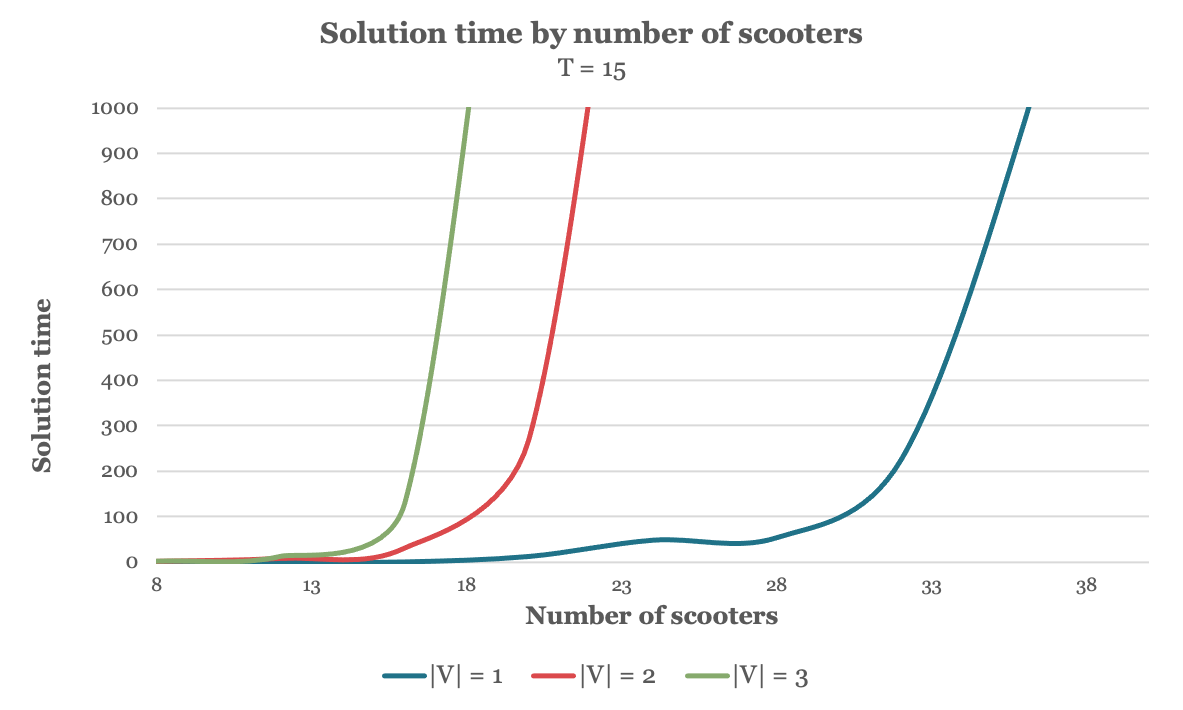
\includegraphics[width=0.8\columnwidth]{Images/Computational Study/size_of_solv_inst.png}
    \caption{Computational complexity with respect to number of e-scooters}
    \label{fig:size_solvable_sens_nodes}
\end{figure}

\textbf{Parameters affecting computational time}
    
The number of service vehicles highly affects the solution time of the model. As seen in \Cref{size_of_solvable_instances}, even for small instances, adding more vehicles increases the complexity significantly. Multiple vehicles introduce the possibility of visiting more locations and consequently more arcs, resulting in lots of combinations to explore. 

In \Cref{fig:size_solvable_sens_time}, the $y$-axis represents the average sum of computational time over instances with a size ranging from 8 to 28 e-scooters. It is important to note that the vertical axis in \Cref{fig:size_solvable_sens_time} is a logarithmic scale of 10. The computational time gets more uniformly distributed over different shift durations when the number of vehicles is incremented. This shows a clear tendency that fleet size is a bottleneck for solving this problem.
\\
\begin{figure}[H]
    \centering
    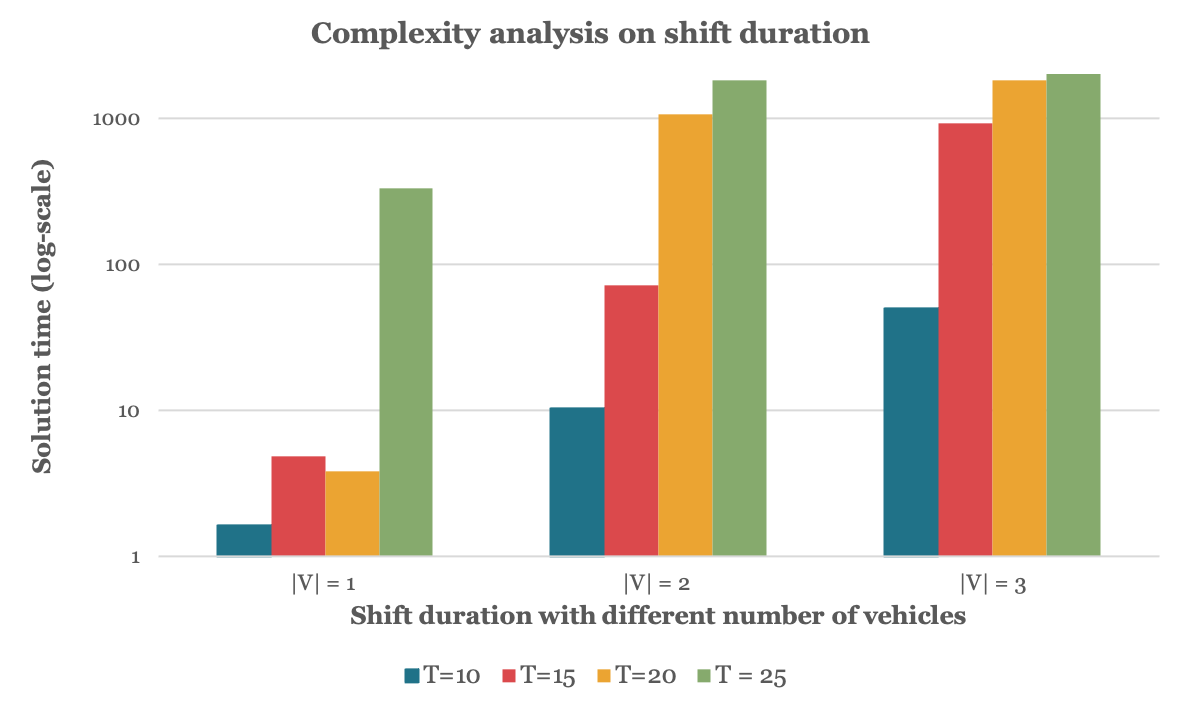
\includegraphics[width=0.8\columnwidth]{Images/Computational Study/sens_shift_dur.png}
    \caption{Computational complexity with respect to shift duration}
    \label{fig:size_solvable_sens_time}
\end{figure}
\Cref{gap_visits} shows the solution gap after one hour of computational time and the percentage of locations visited in the best solution. Number of e-scooters in the system is set to 28. As discussed in \Cref{lit_solution_methods}, \citet{vansteenwegen_iterated_2009} claims that instances where around half of the vertices are visited, are the hardest ones to solve. \Cref{gap_visits} supports this claim, indicating that the model has problems solving instances with a visit percent in the area of 60 percent to optimality within one hour. As previously mentioned, the team orienteering problem (TOP) is a combination of the knapsack problem and the traveling salesman problem (TSP), and thus, longer shift duration leads to a higher visit percentage. When we reach the point of being able to reach all locations, the knapsack constraint is negligible since all rewards can be collected. The problem is then left as a routing problem with an objective function that does not aim to minimize the travel time. 
\\
\begin{table}[H]
    \centering
    \caption{Visit percentage affecting Gap.}
    \begingroup
        \setlength{\tabcolsep}{4pt} % Default value: 6pt
        \renewcommand{\arraystretch}{1} % Default value: 1
    \begin{tabular}{|c|c c|c c|}
        \cline{2-5}
         \multicolumn{1}{c}{} \vline & \multicolumn{2}{c}{V= 2} \vline & \multicolumn{2}{c}{V = 3} \vline\\ \hline
        \textbf{Shift duration} & \textbf{Gap} & \textbf{Visit percent} & \textbf{Gap} & \textbf{Visit percent}  \\ \thickhline
        10 & 0 \% & 20 \% & 29 \% & 26 \% \\
        15 & 16 \% & 51 \% & 91 \% & 63 \% \\
        20 & 68 \% & 63 \% & 66 \% & 69 \% \\
        25 & 27 \% & 91 \% & 24 \% & 97 \% \\
        30 & 23 \% & 94 \% & 22 \% & 100 \% \\
        \thickhline
    \end{tabular}
    \endgroup
    \label{gap_visits}
\end{table}

In summary, the model is able to solve instances of a size between 20-35 e-scooters. The solution time is affected by both the number of service vehicles and the shift duration. An increase in the number of service vehicles drastically increases the computational time. The highest computational time with respect to shift duration is experienced when the optimal solution visits around 60\% of the locations. 
   
\section{Economic Analysis} \label{econ_analysis}

In this section, the aim is to analyze the effect different parameters have on the solution of the model. While \Cref{tech_analysis}
captured the effect on computational time, this section focuses on the economic effects of the solutions.

After conferring with representatives from the Norwegian e-scooter industry, it has come to light that the operators often do not have the capacity nor time to perform rebalancing moves and battery swaps on their whole fleet of e-scooters during a shift. Additionally, the main focus of the operators is to increase the availability of the e-scooters. Thus, it is interesting to examine the effect both longer shifts and additional service vehicles have on the availability, as costs related to these decisions have a substantial effect on the profit of the operators. 

The added availability to a system can be measured by the amount of available battery percentage a solution adds to the state of the e-scooter fleet, represented by the objective function of the standard model. However, the availability of e-scooters cannot only be measured by the battery percentage added to the system, as the allocation of the available e-scooters also has to be taken into account. Thus, the deviation from the ideal state of the system is used as an additional measurement. More specifically, a solution will be evaluated by the squared deviation from the ideal state in each zone. The formula for the total squared deviation is shown in Eq. \eqref{eq:squared_deviation}.  

\begin{eqnarray}
    \displaystyle\sum_{z\in \mathcal{Z}}\left(I_z - \displaystyle\sum_{i\in \mathcal{L}_z} B_i\right)
    ^2\label{eq:squared_deviation}
\end{eqnarray}

This measurement, in contrast to the absolute value of the deviation, is aimed at capturing the fact that a larger deviation from the ideal state in one zone is more severe than a smaller deviation in multiple zones. For example, four zones with a deviation equal to 1 is better than one zone with a deviation of 4. Although the size of the instances do not match real-world scenarios, the parameters have been set to imitate these scenarios as well as possible. 

\subsection{Analysis on the Number of Service Vehicles}

For the operator, the size of the workforce required is an important decision in minimizing cost. Labor is a major variable cost of the operators, and optimizing the use of the labour available could greatly influence their economic performance. Consequently, an analysis with regards to the number of service vehicles needed to maintain a certain level of availability is of great interest. 

\Cref{fig:econ_v} visualizes the value of the objective function for different numbers of service vehicles. The results from the figure are derived from an instance of 20 e-scooters where the service vehicles have a shift duration of 15 minutes. In the figure, four e-scooters added, correspond to a total of four e-scooters with 100\% battery added by the solution. Similarly, an objective function value of 0.5 corresponds to 50\% of battery capacity added and an ideal state of 5 corresponds to 5 e-scooters with 100\% battery capacity. 

\begin{figure}[H]
    \centering
    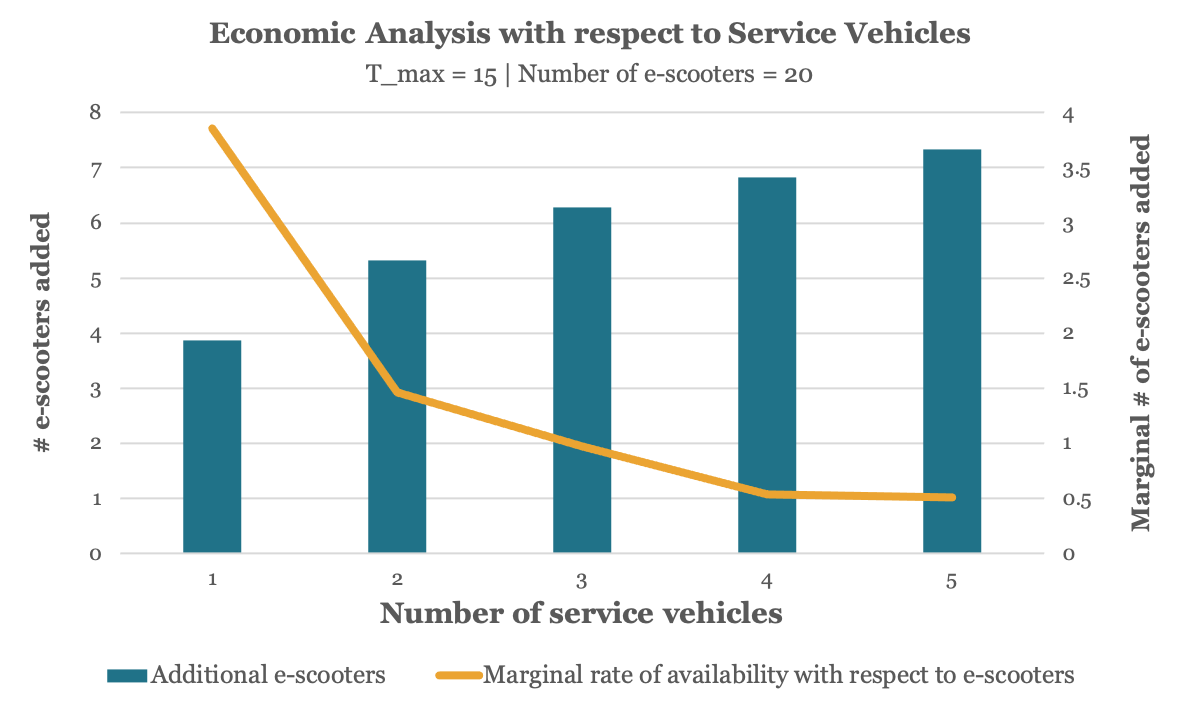
\includegraphics[width=0.8\columnwidth]{Images/Computational Study/econ_vehical_marg.png}
    \caption{The number of e-scooters added for varying numbers of service vehicles.}
    \label{fig:econ_v}
\end{figure}

The marginal rate of availability with respect to the number of service vehicles corresponds to the derivative of the number of e-scooters added for each additional service vehicle. Using three service vehicles instead of two yields an additional 0.97 e-scooters, or 97\% battery capacity. Thus, 0.97 is the marginal rate of additional e-scooters added for three service vehicles. This corresponds to a 18\% increase in the availability of the e-scooter fleet, with the objective function increasing from 5.32 to 6.29. 

The number of e-scooters added for each additional service vehicle decreases as the number of service vehicles increases. The marginal rate of availability is naturally high for low numbers of service vehicles, as each additional service vehicle has multiple locations to visit to perform battery swaps or rebalancing moves. However, this effect decreases as the number of vehicles increases. Additionally, for a fixed shift duration, some of the locations may be very costly to visit, and require the entire shift duration of a service vehicle. This leads to additional vehicles eventually yielding small increases in overall e-scooters added.

\begin{figure}[H]
    \centering
    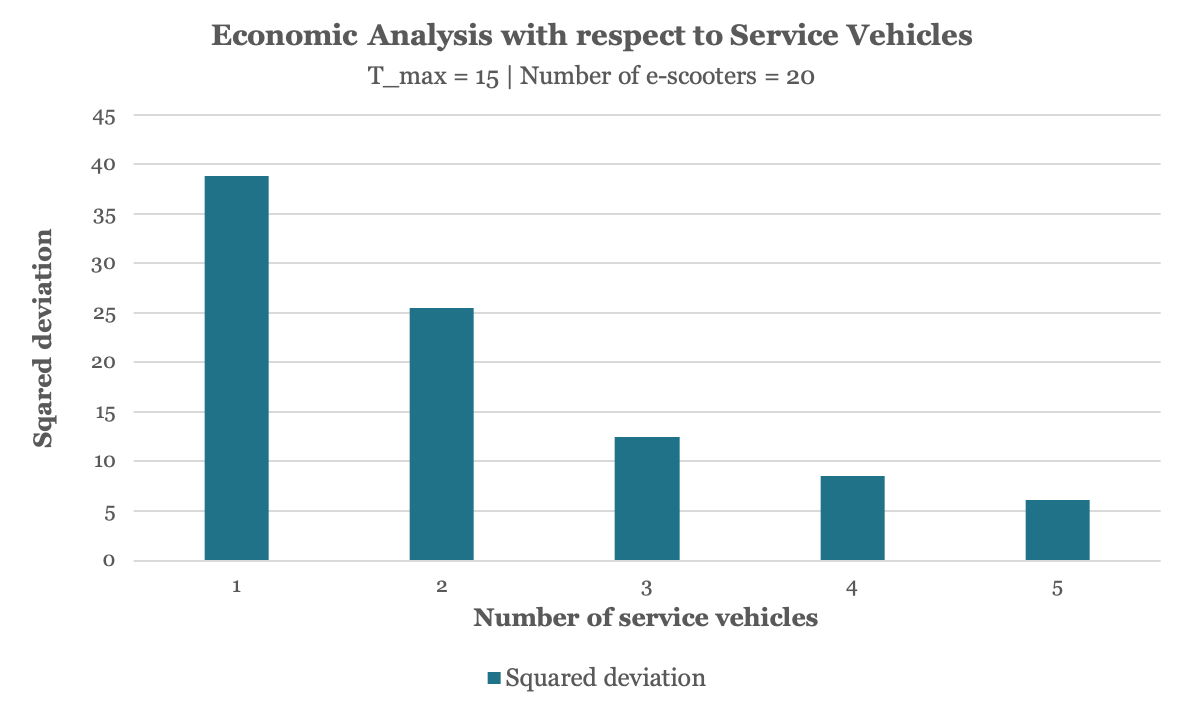
\includegraphics[width=0.8\columnwidth]{Images/Computational Study/econ_vehical.png}
    \caption{The squared deviation for varying numbers of service vehicles}
    \label{fig:econ_v_deviation}
\end{figure}

The squared deviation from the ideal state for each zone follows a similar pattern as the additional e-scooters added, shown in \Cref{fig:econ_v_deviation}. For higher numbers of vehicles, the marginal decrease in deviation declines. As for the analysis of e-scooters added, this is caused by the fact that the previous vehicles already have visited most of the easily reachable locations and performed battery swaps and rebalancing moves at them. However, the squared deviation decreases significantly when adding two and three service vehicles.

Such an analysis of a real-sized problem could assist the operators in making strategic level decisions on the optimal amount of service vehicles needed to maintain a certain availability. An evaluation of the tradeoff between the cost of additional service vehicles and the availability of the e-scooters would have to be made, but indications of the optimal allocation of the service vehicles could greatly influence the decision.

\subsection{Analysis on the Shift Duration}

There is a highly correlated relationship between increasing the number of service vehicles in the model and increasing the shift duration. For every additional service vehicle the total number of available workhours also increases. However, as adding a new service vehicle is a rather large investment, increasing the shift duration could be more feasible for the operators. \Cref{fig:econ_t_max} shows the number of additional e-scooters available for solutions with a varying shift duration. 

\begin{figure}[H]
    \centering
    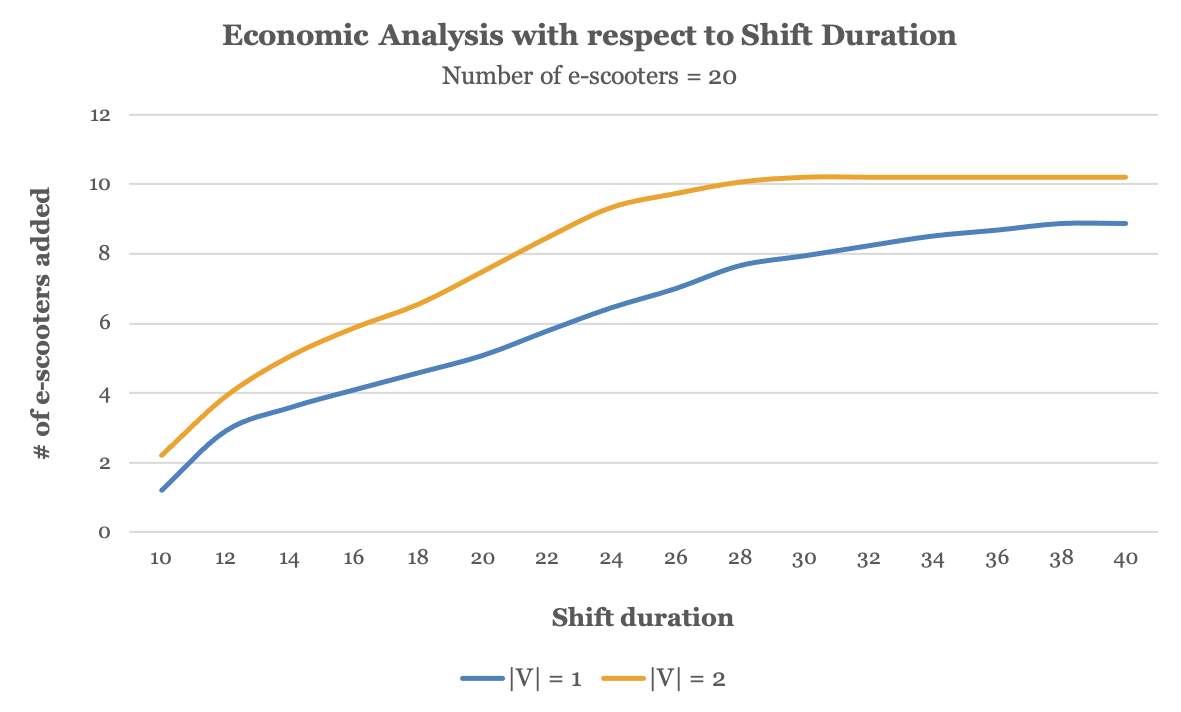
\includegraphics[width=0.8\columnwidth]{Images/Computational Study/econ_shift_dur.png}
    \caption{The number of e-scooters added for varying shift durations.}
    \label{fig:econ_t_max}
\end{figure}

Similarly as for variations in the number of service vehicles, the objective value of the model converges for longer shift durations, as shown in \Cref{fig:econ_t_max}. The explanation is also similar, as the locations in close proximity are the first ones visited, leaving geographically scattered locations to be dealt with for longer shift durations. Consequently, a limit stating when the shift duration is satisfactory can be deducted. The limit for the instance with two service vehicles is somewhat lower than for one service vehicle, as the number of e-scooters added converges faster. This is because the total shift duration for two service vehicles is double that of a single service vehicle. The two instances converge towards different values as a result of the constrained e-scooter capacities of the service vehicles. A single service vehicles does not have the e-scooter capacity to perform all possible rebalancing moves on the same route without performing them in two turns. 

However, the shift duration limit is not only dependent on the number of e-scooters added by the solution. It is also dependent on the significance of the availability of the e-scooter fleet compared to the costs of longer shifts for the operators. Additionally, such a high shift duration might not be feasible for the operator, as labor unions could set an upper limit for the shift duration. Nevertheless, if such an analysis was to be conducted the graphs in \Cref{fig:econ_t_max} could be of great value. 

For the instance with two service vehicles, the squared deviation from the ideal state in each zone decreases rapidly towards 0 as the shift duration increases. However, for an instance with only one service vehicle, the improvement of the squared deviation is not equally distinct. This is partly a result of the fact that a service vehicle in the standard model does not have any incentive to prioritize visits to zones far from its ideal state. This is a quality that a problem-defining implementation of the model should incorporate to mimic real-world scenarios correctly. Consequently, this is incentivized in the alternative model, and discussed further in \Cref{comp_models}.


\section{Comparison of Models} \label{comp_models}
This section compares the standard model presented in \Cref{model} to the alternative model in \Cref{altmodel}. Firstly, the reasoning behind the choice of $\theta$ and $\beta$ for the objective function of the alternative model is provided. Then, a comparison of the computational time and the characteristics of the solutions is given.

\subsection{Parameter Tuning of the Objective Function}
As stated in \cref{reward function}, the parameters $\theta$ and $\beta$ define how the reward function of the alternative model values the number of added scooters in different zones. $\beta$ can be interpreted as the minimum added availability for every added e-scooter. $\theta$, however, describe how much the reward diminish as more e-scooters are added. The values of $\theta$ and $\beta$ used in this report have been found by running the alternative model with a combination of different values for $\theta$ and $\beta$. The evaluation of the solution is based on using the deviation and squared deviation metrics, evaluating the distance from the ideal state. \Cref{fig:assparam_tuning} shows that the deviation vary drastically as  $\theta$ and $\beta$ is changed. The analysis shows that low $\beta$ values and $\theta$ values between $0.5$ and $0.8$ give the lowest deviation. This confirms the interpretation of the parameters discussed. Further in this analysis, $\theta$ and $\beta$ are  set to $0.7$ and $0.05$.

\begin{figure}[h]
     \centering
     \begin{subfigure}{0.45\textwidth}
         \centering
         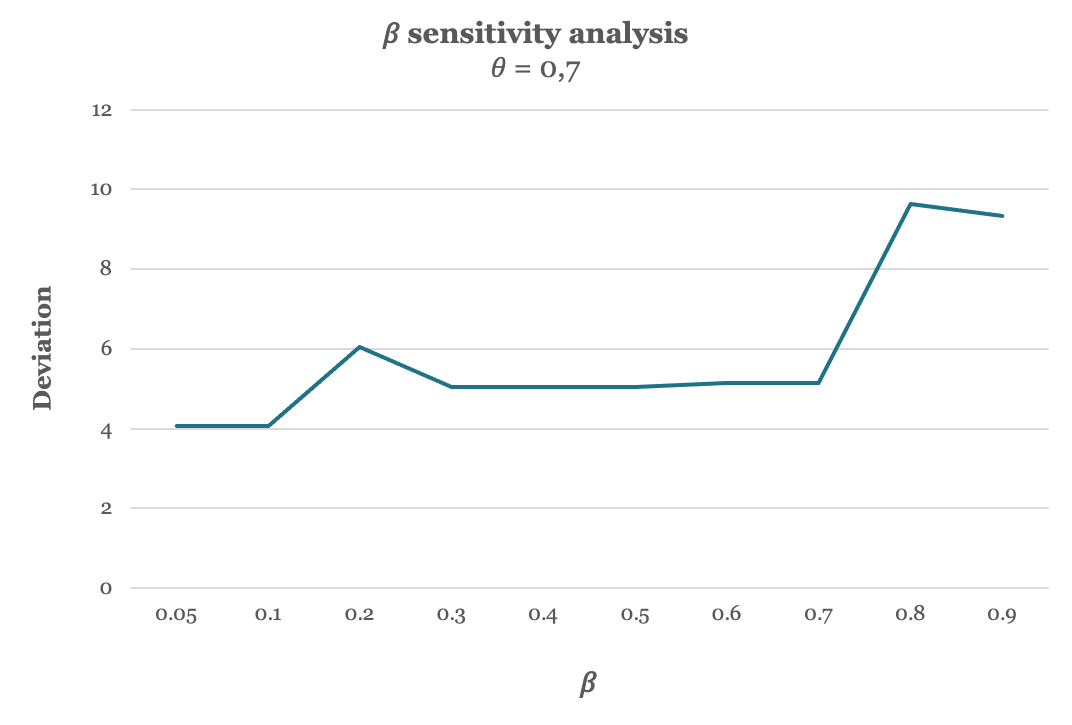
\includegraphics[width=\textwidth]{Images/Computational Study/comp_beta.png}
         \caption{$\theta$ is held constant at $0.7$ while $\beta$ vary from $0.05$ to $0.9$. Deviation increase as $\beta$ increase.}
     \end{subfigure} 
     \hfill
     \begin{subfigure}{0.45\textwidth}
         \centering
         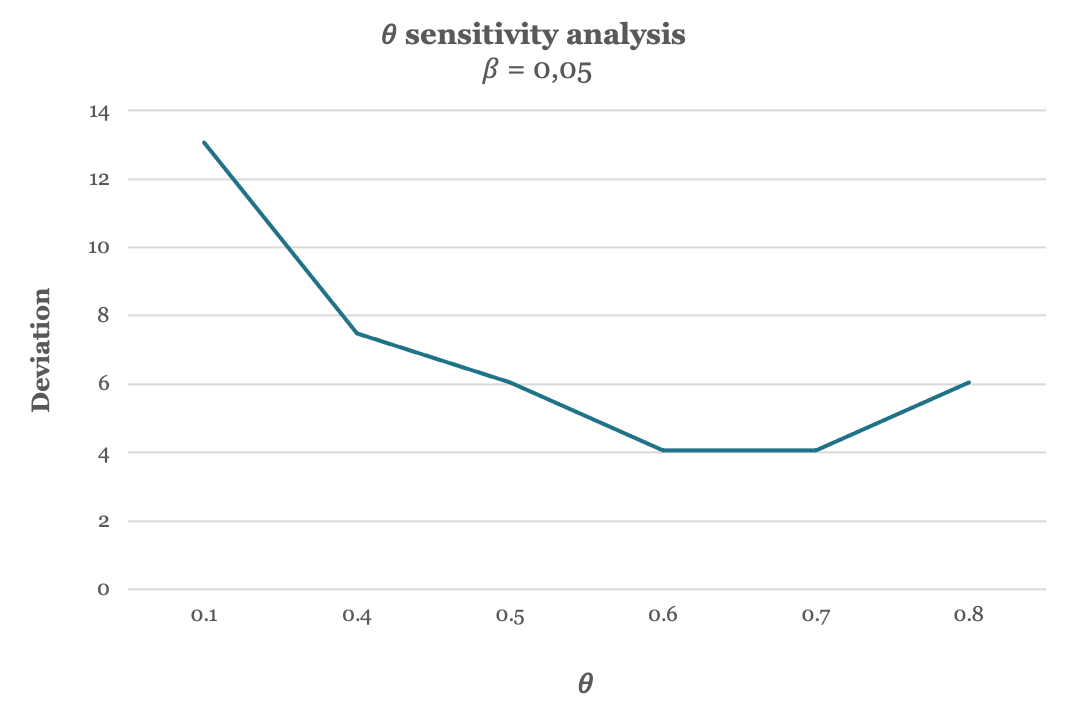
\includegraphics[width=\textwidth]{Images/Computational Study/comp_theta.png}
         \caption{$\beta$ is held constant at $0.05$ while $\beta$ vary from $0.1$ to $0.8$. The plot reaches a minimum for $\theta$ values between $0.5$ and $0.8$.}
     \end{subfigure}
     \caption{Sensitivity analysis on $\theta$ and $\beta$.}
     \label{fig:assparam_tuning}
\end{figure}

However, these parameters can be set by the operator to fit their preferences. Looking at \cref{tab:alphabeta_data} some general patterns can be observed. High values of theta gives generally low deviation as the model values each e-scooter highly. Combining a high theta with a low beta will give initial e-scooters handeled in a high reward and then reduce the reward drastically as we introduce more e-scooter. 
\\
\begin{table}[H]
    \centering
    \caption{All instances where solved to optimality}
    \begin{tabular}{|c c | c c c |}
        \hline
        $\theta$ & $\beta$ & Deviation Squared & Visit \% & Solution Time \\
        \hline
        0.1 & 0.05 & 13.1 & 5\% & 1.9 \\
        0.7 & 0.05 & 4.1 & 30\% & 7.0 \\
        0.1 & 0.5 & 6.1 & 30\% & 9.4 \\
        0.8 & 0.5 & 5.1 & 45\% & 26.5 \\
        0.1 & 0.9 & 9.2 & 70\% & 404.8 \\
        0.9 & 0.9 & 9.7 & 55\% & 295.1 \\
        \hline
    \end{tabular}
    \label{tab:alphabeta_data}
\end{table}

\subsection{Comparison of Size of Solvable Instances}
\Cref{fig:SizeOfSolvableInstancesAltModel} shows that the standard model outperforms the alternative model in terms of solution time. However, looking at \cref{tab:alphabeta_data}, increasing $\beta$ the model visits more locations, increasing the computational time. Therefore, for some low $\beta$ values, the alternative model is faster due to having fewer locations to visit. This is illustrated by the red line in \Cref{fig:SizeOfSolvableInstancesAltModel}. However, the figure illustrates that the standard model is able to solve bigger instances. 

\begin{figure}[h]
    \centering
    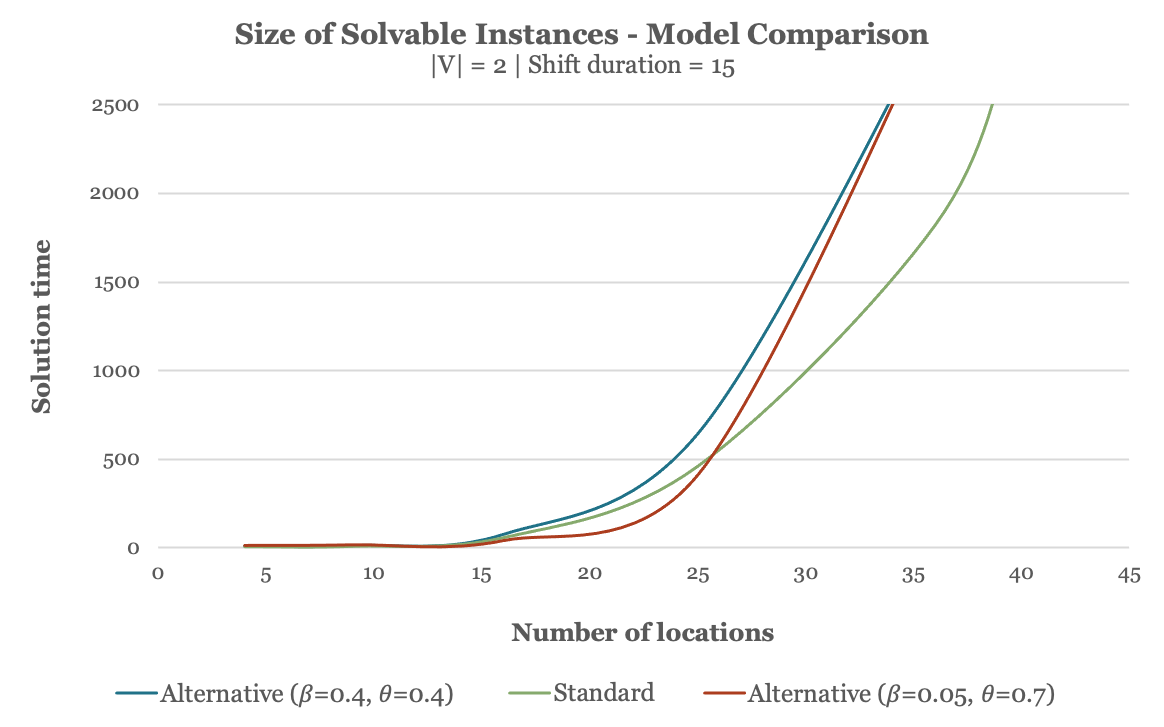
\includegraphics[width=0.9\textwidth]{Images/Computational Study/comp_loc.png}
    \caption{Solution time of increasing number of locations. The blue and red line show solution time for two different configurations of $\beta$ and $\theta$, while the green line shows the same for the standard model}
    \label{fig:SizeOfSolvableInstancesAltModel}
\end{figure}

\subsection{Comparison of Solutions}
As discussed when presenting the alternative model, the main difference between the models is the objective function. The standard model value an action independently of which zone it belongs to. The alternative model, however, values performing an action in a zone far away from its ideal state more than those with a sufficient number of e-scooters already. This is done to end up closer to the ideal state. Hence, a comparison of solutions by observing the objective value is not sufficient.

As the ideal state is a common goal for both models it is be a performance indicator in our comparison. This also makes sense in the context of reaching maximum availability as less deviation leads to more available e-scooter. The squared deviation is a good measure for describing the deviation from the ideal state, as described in \Cref{econ_analysis}. \Cref{deviation_comparison_a_and_s} summarizes the squared deviation between the models for the instances in \Cref{computational_preliminary}. The data clearly shows, as expected, that the alternative model has a lower deviation squared. 
\\
\begin{table}[H]
    \centering
    \caption{Comparison of deviation between the standard and the alternative model}
    \begin{tabular}{c c c}
        \thickhline
        & \multicolumn{2}{c}{\textbf{Deviation Squared}}  \\
        \thickhline
        \textbf{Model type} & Standard & Alternative \\
        \hline
        \textbf{Instance 1} & 2.948 & 2.045 \\
        \textbf{Instance 2} & 2 & 0.533 \\
        \textbf{Instance 3} & 7.78 & 4.272 \\
        \thickhline
    \end{tabular}
    \label{deviation_comparison_a_and_s}
\end{table}

The two figures, \Cref{fig:comp_study_comp_models_S} and \Cref{fig:comp_study_comp_models_A}, illustrate the main difference in the solutions of the alternative and the standard model. The alternative model is incentivized to visit more zones and do more rebalancing moves than the standard model as it is less rewarded for swapping batteries in zones with an excess of e-scooters. This can be seen in \Cref{fig:comp_study_comp_models_S} where the standard model mostly swaps batteries in the zones already containing multiple e-scooters. It has no incentive to visit locations in all zones as it gets the same reward for swapping one additional battery in an already full zone and performing a rebalancing move to a zone in demand of e-scooters. The alternative model, however, visits the locations in zone 1 as well. This is because it is not rewarded for performing more battery swaps of e-scooters in zone 4. \cref{tab:solution comparison data} show the deviation before and after for the solutions of both models. 
\\
\begin{figure}[H]
    \centering
    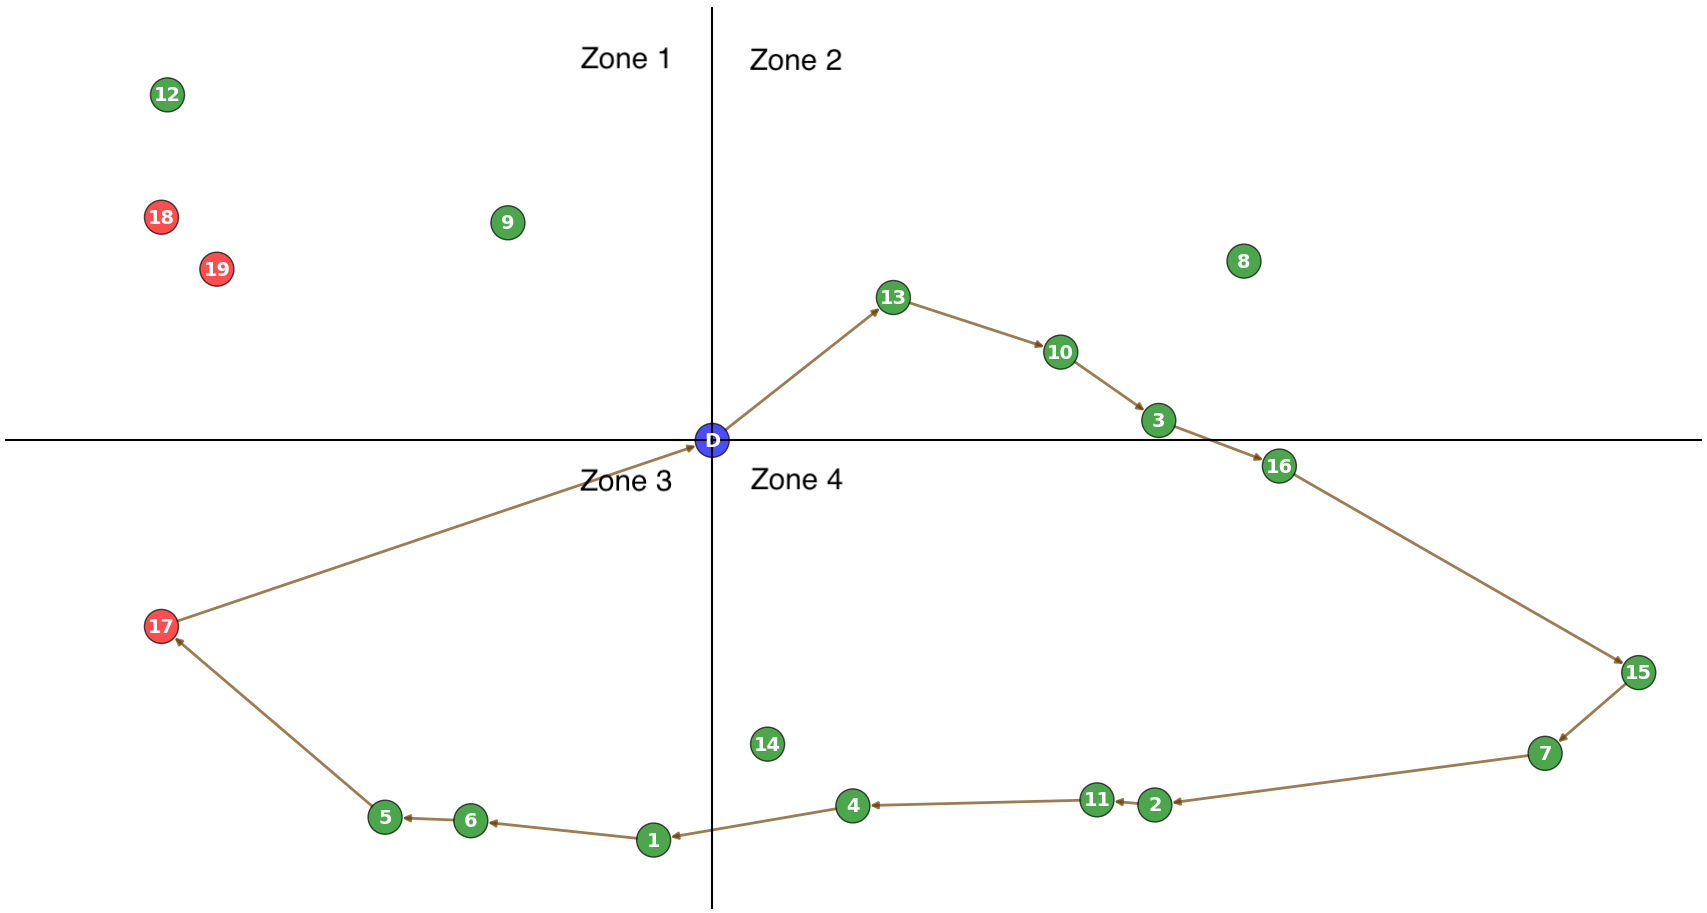
\includegraphics[width=0.8\textwidth]{Images/Computational Study/comp_S.png}
    \caption{Solution created by the standard model. This instance has an ideal state of four e-scooters per zone using a single service vehicle. The route chosen visit many nodes in zone 4 even though this zone already have too many e-scooters available.}
    \label{fig:comp_study_comp_models_A}
\end{figure}
\begin{figure}[H]
    \centering
    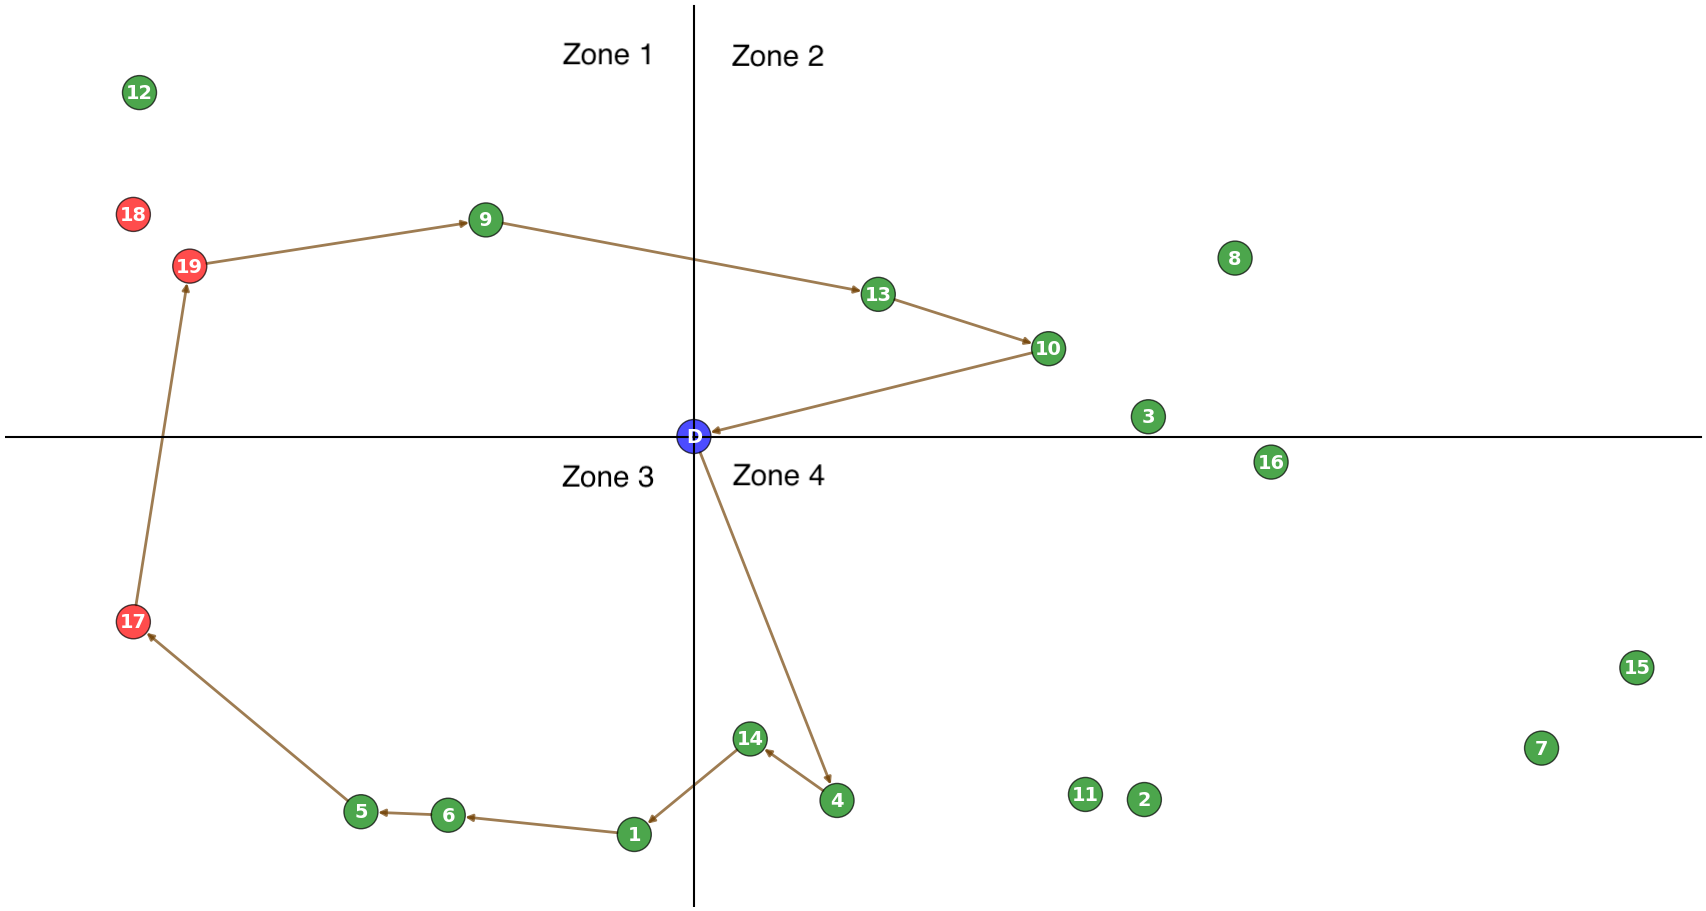
\includegraphics[width=0.8\textwidth]{Images/Computational Study/comp_A.png}
    \caption{Solution created by the alternative model model. This instance has an ideal state of four e-scooters per zone using a single service vehicle. The route chosen first performs pick-ups in zone 4 where there is an excess demand. It then delivers these nodes in zones 3 and 1 where there is a demand for available e-scooters.}
    \label{fig:comp_study_comp_models_S}
\end{figure}

\begin{table}[H]
    \centering
    \caption{Deviation from ideal state before and after operation for both models. The numbers in \textit{italic} indicate a negative deviation meaning that the zone has more e-scooters than the ideal state.}
    \begin{tabular}{c | c c | c c}
        \thickhline
         \multicolumn{1}{c}{} & \multicolumn{2}{c}{\textbf{Standard Model}} \vline & \multicolumn{2}{c}{\textbf{Alternative Model}}\\
        \thickhline
        \textbf{Zone} & Deviation Before & Deviation After & Deviation Before & Deviation After  \\
        \hline
        \textbf{1} & 3.04 & 3.04 & 2.5 & 1.56  \\
        \textbf{2} & 1.4 & 0.33 & 2.5 & 0.34  \\
        \textbf{3} & 2.88 & 0 & 2.5 & 0  \\
        \textbf{4} & \textit{0.47} & \textit{1.78} & 2.5 & 0.68  \\
        \hline
        \textbf{Total} & 7.79 & 5.15 & 7.79 & 2.55 \\
        \thickhline
    \end{tabular}
    \label{tab:solution comparison data}
\end{table}
